\chapter{绪论}

\section{引言}

软件定义网络(Software Defined Network,SDN)将网络控制平面和数据平面进行分离,并通过逻辑上集中式的SDN控制器向上层应用提供网络全局视图,使灵活、高效的网络管理变得可能~\cite{mckeown2008openflow,feamster2013road,b4}。对于底层数据平面中的网络设备,通过南向接口(例如OpenFlow协议~\cite{mckeown2008openflow}),SDN控制器上的应用可以对其进行配置,进而控制网络中数据包的传输。然而,让上层应用直接调用底层网络设备的低级配置接口对其进行配置,则会导致系统非常容易出错,影响可拓展性。因此,研究人员在SDN中提出高级编程模型的概念~\cite{foster2011frenetic,maple,reich2013modular},对上层应用提供对网络配置的高级抽象接口,并自动地将上层应用表达的高级抽象网络策略转化为底层网络设备的低级配置。然而,随着SDN概念的普及,以及底层网络设备技术的迅速发展,SDN高级编程模型不断迎接着新的挑战。

一方面,随着SDN概念的普及,上层应用希望SDN高级编程模型提供的高级抽象接口可以不断地支持新的特性。从最原始的对单个交换机的配置,到可以对网络中多个交换机的配置,再到可以对网络中交换机和特定网络功能节点(如防火墙)的统一配置。从对网络管理的意图(intent)~\cite{berde2014onos},到高级SDN程序(即逻辑上可以应用于网络中所有数据包的onPacket函数),再不断地丰富高级SDN程序的语法(如支持循环结构,支持路由代数~\cite{gao2018t}等)。这些上层应用迫切希望的新的特性,给高级编程模型所提的自动地生成底层网络设备的低级配置带来了巨大挑战。

另一方面,随着底层网络设备技术的迅速发展,底层网络设备在不断变得高效、灵活的同时,其架构也变得越来越复杂。从OpenFlow1.0~\cite{openflow1}的单流表架构,到OpenFlow1.1~\cite{openflow1-1}的多流表流水线架构,再到协议无关并可自定义的多流表流水线架构的P4~\cite{P4}。最初的单流表架构虽然简单,但由于多个匹配域的叉乘(cross-product),单流表架构并不高效~\cite{openflow1-3-1}。多流表流水线架构解决了匹配域的叉乘问题,但其架构也变得复杂从而影响流表规则的下发:要考虑给哪一个流表下发。P4的协议无关并可自定义的多流表流水线架构实现了非常灵活的网络配置,但使用时不光要考虑流表规则的下发,而且(实际上要先于流表规则下发)要考虑生成多流表流水线结构。支持有状态操作的可编程交换机~\cite{moshref2014flow,bianchi2014openstate}其强大的灵活性也伴随着复杂的架构。这些新诞生的底层网络架构同样给高级编程模型带来了巨大挑战。

随着高级抽象接口支持的特性越来越多,底层网络设备架构变得越来越复杂,两者之间结构的差异也会变得越来越大。而SDN高级编程模型始终需要考虑的问题则是,如何高效地填充两者之间不断变大的鸿沟,即尽可能地将上层应用表达的高级抽象网络策略转化为符合底层网络设备架构的高效的低级配置。

在这章中,我们先从面向单交换机和面向全网络两个大方向进行研究背景介绍。其中对于面向单交换机,我们先介绍可编程数据通路(datapath)的研究,再介绍面向单交换机编程模型的研究;对于面向全网络,我们先介绍面向一般网络编程模型的研究,再介绍针对特定网络编程模型的研究。再结合介绍内容,给出论文中主要的研究挑战以及相关解决方案。最后给出论文整体架构。


\section{研究背景:面向单交换机}

\subsection{可编程数据通路的研究背景}

可编程数据通路的研究可以分为两大类:基于硬件的可编程数据通路,基于软件的可编程数据通路。

\para{基于硬件的可编程数据通路}:灵活的数据包分类(即可以利用通配符对数据包匹配域的任意组合进行匹配)是实现可编程数据通路的基础。基于TCAM的三元匹配功能(即0,1,x),可以非常高效地实现数据包分类~\cite{yu2005efficient,lakshminarayanan2005algorithms,song2005efficient}。然而,由于TCAM的电力消耗,以及占用的电路空间等问题,TCAM不具备很好的可拓展性。Naous等人~\cite{naous2008implementing}将数据通路中的匹配表分为准确匹配和通匹配,并分别利用SRAM和TCAM进行实现。最终他们在NetFPGA平台上实现了OpenFlow交换机。Jiang等人~\cite{jiang2011scalable}基于决策树的数据包分类算法,在单个FPGA上放置了10K条可以支持5个匹配域的规则或1K条可以支持12个匹配域的规则。

由于单纯利用交换机芯片无法实现灵活的数据包处理,研究者开始考虑利用交换机中的其他资源(如CPU)来处理一部分数据包操作。Luo等人~\cite{luo2009accelerating}利用基于网络处理器的加速卡实现OpenFlow交换机,并降低了百分之二十的网络数据包延迟。Lu等人~\cite{lu2012using}利用CPU来辅助ASIC交换机对数据流的处理。具体来说,他们利用CPU实现基于流转发的大容量匹配表以及利用DRAM存储网络中突发数据包。Mogul~\cite{mogul2012hey}等人利用CPU实现交换机中的软件定义计数器,以达到对计数器相关信息的灵活操作。类似的,他们利用DRAM存储计数器,并通过CPU对其进行更新操作。数据包匹配后会在buffer中存储匹配记录,然后CPU根据buffer记录更新DRAM中数据。

对于单流表匹配结构对流表容量要求较大(由于匹配域叉乘),使用起来并不高效等问题,研究人员考虑用多流表流水线作为可编程数据通路的基本结构。OF-DPA~\cite{OF-DPA}是Broadcom提出的OpenFlow数据平面抽象。OF-DPA与OpenFlow v1.3.4兼容,其底层为多个具有固定匹配域流表的流水线结构。PicOS~\cite{PicOS}与OF-DPA类似,在底层为多个具有固定匹配域流表的流水线情况下,向上兼容OpenFlow协议。FlowAdapter~\cite{pan2013flowadapter}设计了具有三层的交换机架构。其中上层为OpenFlow软件数据平面,并通过中间的Flow Adapter转化为底层的OpenFlow硬件数据平面。

对于上面所述的多流表流水线架构,用户只可以下发流规则,不可以更改流水线结构。因此,为了追求更灵活的可编程数据通路,研究人员开始考虑自定义的多流表流水线架构。Forwarding Metamorphosis~\cite{rmt}提出RMT架构,表示Reconfigurable Match Tables。RMT架构包含ingress processing、egress processing、以及中间的队列结构。其中processing由parser、deparser、以及中间的多个stage组成。一个流水线上的逻辑流表可以由一个或多个stage共同实现,因此RMT可以灵活地实现具有不同结构的多流表流水线。同时其parser也可以自定义。最终,RMT实现了协议无关可自定义的多流表流水线架构。dRMT~\cite{chole2017drmt}删除了RMT中stage与流表的绑定关系,即任何stage可以访问任何流表;删除了stage与stage的依赖关系,即数据包可以进入任意stage而无需经过前面的stage,实现了更灵活更高效的数据包处理。为了考虑更丰富的数据包操作,PISA~\cite{pisa}概括了RMT架构并实现了更灵活的数据包操作指令(atoms)。OpenState~\cite{bianchi2014openstate}考虑了有状态的操作。

\para{基于软件的可编程数据通路}:Linux内核~\cite{linux},DPDK~\cite{dpdk},Netmap~\cite{rizzo2012netmap},Click~\cite{kohler2000click}等工作需要对底层实现具有相当的了解才能在上面构造软件交换机,这对网络程序员需要快速适应这些平台并开发新特性增加了困难。Open vSwitch(OVS)~\cite{pfaff2015design}考虑了向其添加流表规则的接口,但不可以自定义地配置协议以及操作。Oko~\cite{chaignon2018oko}通过Berkeley Packet Filter (BPF) 对Open vSwitch进行拓展,使其可以支持有状态过滤器。Pisces~\cite{shahbaz2016pisces}是一个可编程的协议无关的软件交换机,程序员可以在上面通过P4语言进行配置,并可以输出以OVS为目标的底层代码。


\subsection{面向单交换机编程模型的研究背景}

2006年,IETF网络配置工作组提出了NETCONF~\cite{enns2006netconf}作为用于修改网络设备配置的管理协议。NETCONF允许网络设备发布可通过其发送以及接受可扩展配置数据的API。另一种广泛部署的网络设备管理协议是SNMP~\cite{hare2011simple}。SNMP使用结构化管理接口(SMI),以获取存储于管理信息库(MIB)中的数据。通过SNMP,网络管理员可以改变MIB中的变量以修改配置设置。

OpenFlow~\cite{mckeown2008openflow}是目前SDN中所使用最广的南向接口标准。OpenFlow对于支持OpenFlow转发设备提供了一个共同说明,以及对于SDN数据平面和控制平面之间的通信通道提供了标准。从OpenFlow1.1~\cite{openflow1-1}开始,OpenFlow标准增加了多表、组表以及流水线处理技术。对于支持OpenFlow多流表交换机,当数据包到达时,和第一个流表中的流项进行匹配。匹配成功时执行相应操作,可以是应用指令或者跳转至指定其他流表,实现数据包在多个流表之间的转移。组表可以用来实现多播。从OpenFlow1.3~\cite{openflow1-3}开始增加Meter表,用来实现简单的QoS操作。

OVSDB~\cite{pfaff2013open}的设计是向Open vSwitch提供一个高级的管理接口。除了OpenFlow的基本配置流表的能力外,通过OVSDB可以创建多个虚拟交换机的实例,以及向交换机接口设置QoS策略。

目前面向多流表流水线的交换机配置语言包括Concurrent Netcore~\cite{schlesinger2014concurrent}以及P4~\cite{P4}。Concurrent Netcore可以用来指定路由策略以及多流表中数据包处理的顺序。P4作为目前占有统治地位的配置自定义多流表流水线的语言,P4不光可以支持自定义的流水线结构,而且可以自定义数据包的parser以实现协议无关的流水线。


与P4需要手动地指定每一个流表的格式以及流水线的结构不同,Packet transactions~\cite{sivaraman2016packet}向用户提供了一个高级编程模型,可以用来自动地生成底层数据通路的结构。通过该高级编程模型,用户可以编写onPacket函数并提交给Packet transactions,后者会自动生成底层数据通路结构以及配置。在生成底层数据通路结构时,Packet transactions会合并用户onPacket函数中的语句。


\section{研究背景:面向全网络}


\subsection{面向一般网络编程模型的研究背景}


一般网络这里是相对特定网络(如车联网等)而言的概念。我们考虑的面向一般网络的编程模型不会对网络实现的功能以及应用场景进行限制。

在1990年代中期,Active Networking~\cite{tennenhouse1997survey,tennenhouse1996towards}提出了通过可编程网络基础架构,可以实现定制化的服务。主要有两种方法
被考虑:1. 通过用户可编程交换机并使用in-band负责数据传输,out-of-band负责管理信道;2. 将需要执行的程序附带在数据包上,并在交换机或路由器上执行对应的程序。

基本SDN控制器如\cite{gude2008nox,erickson2013beacon,medved2014opendaylight,shalimov2013advanced},向下通过OpenFlow协议与底层交换机通信,获取网络状态信息并传给控制器上的应用程序。通过响应式模式,上层应用收到底层数据包后,进行相关处理,再通过控制器提供的接口对相关网络设备进行配置。ONOS~\cite{berde2014onos}提供意图的方式对网络中数据流的传输进行控制。

具有SDN编程抽象的系统如FML~\cite{hinrichs2009practical},一种基于流的管理语言提供了高级编程模式来指定网络安全相关配置。Onix~\cite{koponen2010onix}引入了NIB(Network Information Base)抽象,以便应用程序通过读写存储在NIB中的键值对来修改流表。Frenetic~\cite{foster2011frenetic},Pyretic~\cite{reich2013modular},Nettle~\cite{voellmy2011nettle},提供了SDN编程语言。其中Frenetic的NetCore支持特定的策略组合形式,如信息收集和数据流控制。Pyretic拓展了Frenetic提供了基于模块化的SDN编程语言。Nettle则是基于函数式相应式编程(FRP)对网络进行控制。Maple~\cite{maple}提出了基于算法式的SDN编程语言,并提供对数据包的读、测试等基本API。通过记录数据包执行的踪迹,构建踪迹树,然后基于踪迹树自动生成底层流表。McClurg等人~\cite{mcclurg2016event}提出网络事件结构的模型,保证了在事件到达时对网络状态的更新过程中也可以满足的指定的不变性质。

SNAP~\cite{snap}考虑将高级SDN程序转化为多个有状态交换机的配置。但是其编程模型为One-Big-Switch模型,即用户无法指定数据包在网络传输的具体路径。


\subsection{面向特定网络编程模型的研究背景}

我们这里对特定网络分为三种情况:1. 交换机和中间盒(或NFV)的混合网络;2. 实现特定功能的网络(如Paxos);3. 针对特定场景的网络(如车联网,物联网等)。

\para{混合网络}:Qazi等人~\cite{qazi2013simple}通过SDN保证数据流可以正确地传过事先规定好的中间盒序列。Fayazbakhsh等人~\cite{fayazbakhsh2014enforcing}解决了当中间盒对数据包头进行修改后,数据包仍然可以按照指定路径进行转发。Trident~\cite{gao2018t}考虑利用网络中间盒可以处理数据包更高层信息的功能,设计统一的高级编程模型,使网络数据包的传输可以依赖更高层信息(如数据包对应流的http信息)。为了实现类似的功能(即数据包根据高层信息进行转发),Mekky等人~\cite{mekky2014application}采取拓展Open vSwitch的方法,使交换机存储状态信息。

\para{实现特定功能的网络}:通过利用可编程交换机,一些传统的分布式算法可以高效地在网络中实现。NetPaxos~\cite{dang2015netpaxos,dang2016paxos}利用P4语言对可编程交换机进行配置,使其分别扮演Paxos~\cite{lamport2001paxos}的acceptor,coordinator等角色,通过订制包头的数据包在交换机之间的传输,实现分布式一致性算法。基于类似的想法,Netcache~\cite{jin2017netcache}和Netchain~\cite{jin2018netchain}则利用可编程交换机流表的性质,将键值对存储在网络中,实现分布式键值对存储。Typhoon~\cite{cho2017typhoon}利用底层DPDK数据平面,实现基于SDN的实时大数据流处理框架。Beckett等人~\cite{beckett2016don}针对BGP场景,将BGP路由的约束转化为底层交换机的配置。

\para{特定场景网络}:Zhu等人~\cite{zhu2018sdn}考虑利用SDN技术实现车联网中紧急消息的快速分发功能。Hare等人~\cite{hare2012policy}设计一个集中式的策略框架来管理车辆网络的光谱资源来保证用户需要的数据传输性能。Mobile fog~\cite{hong2013mobile}提出面向物联网的编程模型。Mobile fog中的一个应用由多个进程组成,每个进程映射到网络中的一个节点,如核心节点,fog节点,边缘节点。进而这些进程根据节点之间的层级关系,也组成一个逻辑上的层级关系(如父子节点关系)。通过层级关系,进程之间可以发送数据,共同完成任务。


\section{论文研究挑战}

根据上节对研究背景的叙述,我们把本论文研究的挑战主要分为两部分: 面向单交换机编程模型的研究和面向全网络编程模型的研究。而每一部分都有两个基本问题:SDN程序数据平面实现问题和针对特定场景情况的优化问题。其中实现问题是指:给定一个SDN程序,一个数据平面是否可以正确表达该SDN程序。正确是指:对于任意数据包,SDN程序对数据包返回的结果和数据平面对数据包返回的结果一致。下面我们针对上述的两部分来具体说明论文研究挑战。

第一,在面向单交换机编程模型的研究中,已有的相关工作可以分为如下:1. 通过低级配置接口生成具有固定结构(如单流表或OF-DPA)数据通路的配置;2. 将高级程序转化为具有可定制结构(如RMT)数据通路的配置。但是缺少将高级程序转化为具有固定结构数据通路的配置的相关工作。而在转化之前,需要考虑的是该固定结构数据通路是否可以实现高级程序。因此,如何判断一个高级SDN程序是否可以在具有固定结构数据通路上实现,是一个挑战。除此之外,当SDN程序具有循环结构时,如何将该SDN程序实现在可定制结构数据通路上并没有相关工作。因此高级SDN程序中循环结构在可定制结构数据平面的高效实现,是一个挑战。

第二,在面向全网络编程模型的研究中,对于一般网络,大量工作是以响应式模式(即不会主动生成配置)对网络进行管理,因此效率并不高。SNAP实现了主动编译生成数据平面配置,但其程序并不灵活。因此,给定一个高级灵活的SDN程序,如何生成面向全网络的数据平面配置是一个挑战。除此之外,针对不同场景,如软件定义联合~\cite{mishra2017comparing}网络的低时延要求,以及车联网中车的移动性要求,如何优化数据平面配置是一个挑战。

\section{论文研究内容}

针对上一节中探讨的两方面的挑战,本文进行有针对性的研究,主要分为以下五个部分:

第一,针对判断高级SDN程序是否可以在具有固定结构数据通路实现问题,提出了将高级SDN程序和底层数据通路进行统一的特征空间。并将判断问题转化为空间中的比较问题,形成系统的数据通路编程容量理论。

第二,针对高级SDN程序中循环结构在可定制结构数据通路的高效实现问题,提出了重复软件流水线转换。通过转换,在计算循环结构的最佳数据通路结构时显示出更高的效率。

第三,针对高级灵活的SDN程序面向全网络数据平面实现问题,当网络节点全部为可编程交换机时,提出将程序拆分并部署到不同交换机的方案,并算出给定目标下的最优部署;当网络节点存在固定功能节点时(如防火墙),提出程序正确性的定义,并通过系统路径约束的概念保证程序的正确。

第四,针对软件定义联合网络的具体场景,设计高级编程系统,并基于共享本地状态的方法,优化系统性能:降低数据传输时延,提高传输带宽。

第五,针对车联网的具体场景,提出软件定义车联网的架构以及编程框架。考虑车联网中车移动性特点,提出优化的规则下发方法,减少生成的规则数量。

\begin{figure}[h!]
    \centering
    % \vspace{-0.1in}
    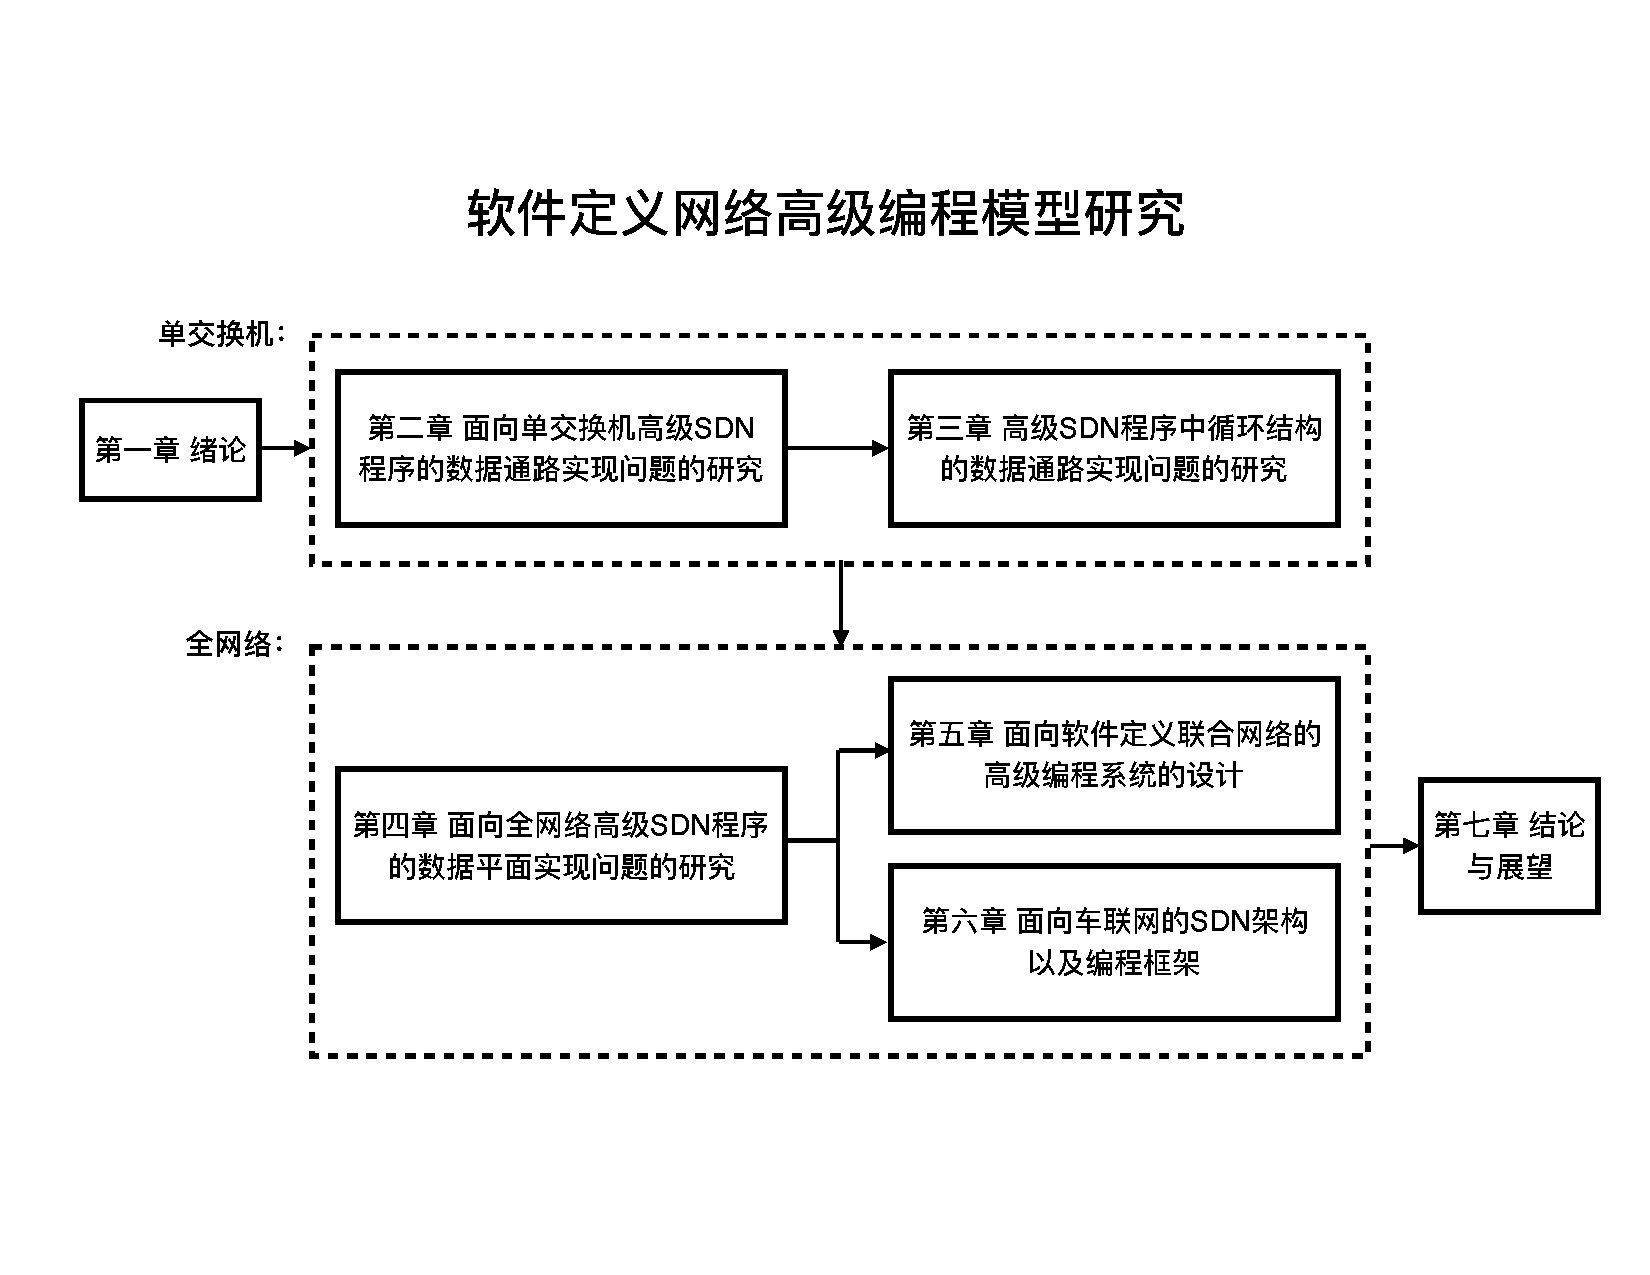
\includegraphics[width=0.9\linewidth]{figures/intro-fig1.pdf}
    % \vspace{-0.1in}
    \caption{论文框架}
    % \vspace{-0.1in}
    \label{intro:fig1}
\end{figure}


\section{论文结构}

如图~\ref{intro:fig1}所示,本论文总共由七部分组成:第一章为绪论,先介绍了目前软件定义网络高级编程模型研究的背景。并根据背景给出论文挑战,最后列出论文内容。

第二章,第三章均为面向单交换机情况。其中,第二章研究面向单交换机的高级SDN程序数据通路实现问题,并给出特征空间以及数据通路编程容量理论。待第二章的基本实现问题讨论完后,第三章考虑高级SDN程序中循环结构,并给出循环结构在可定制结构数据通路的高效实现方法。

第四章,第五章,第六章均为面向全网络情况。其中,第四章研究面向全网络的高级SDN程序数据通路实现问题。待第四章的基本实现问题讨论完后,第五章考虑针对软件定义联合网络的数据平面优化,第六章考虑软件定义车联网架构以及编程框架。

最后,第七章总结了研究内容并对未来工作进行展望。在正文之后,附上参考文献,博士期间个人论文发表情况。
